
The method we employed to use \CP\ can be visualized in a four part
fashion, as depicted in \refFigure{fig:genView}. The first part, in
the upper level of the figure, shows the Selector, which selects a
set of values for the inlining parameters based on a strategy. The
second part, on the left, shows the Combined Profiling (\CP) process
applied to a program. The third part, at the bottom of the figure,
shows the execution test of a compiled program. And, in the center
of the figure we have the compiler.

\begin{figure}
  \centering
  \includegraphics[width=0.50\linewidth]{Figures/genView}
  \caption{Generic view of the method}
  \label{fig:genView}
\end{figure}

We can use this method for parameter tuning, and also for a machine
learning approach trying to define the best set of parameters for
throughput or for latency. The process remains the same, we just have
to define properly what is a point of measure. More details on the
\CP\ profiling in \refFigure{fig:CPview}, whereas in \refFigure{CP:simple}
the simplified view is presented, the hatched area marks the \CP\
compiler; and in \refFigure{CP:expanded} the \CP\ compiler is shown in
more detail.

\begin{figure}
  \centering
  
  \begin{minipage}[t]{\linewidth}
    \subfigure[Simplified view of the process] {
      \begin{minipage}[b]{0.45\textwidth}
        \centering
        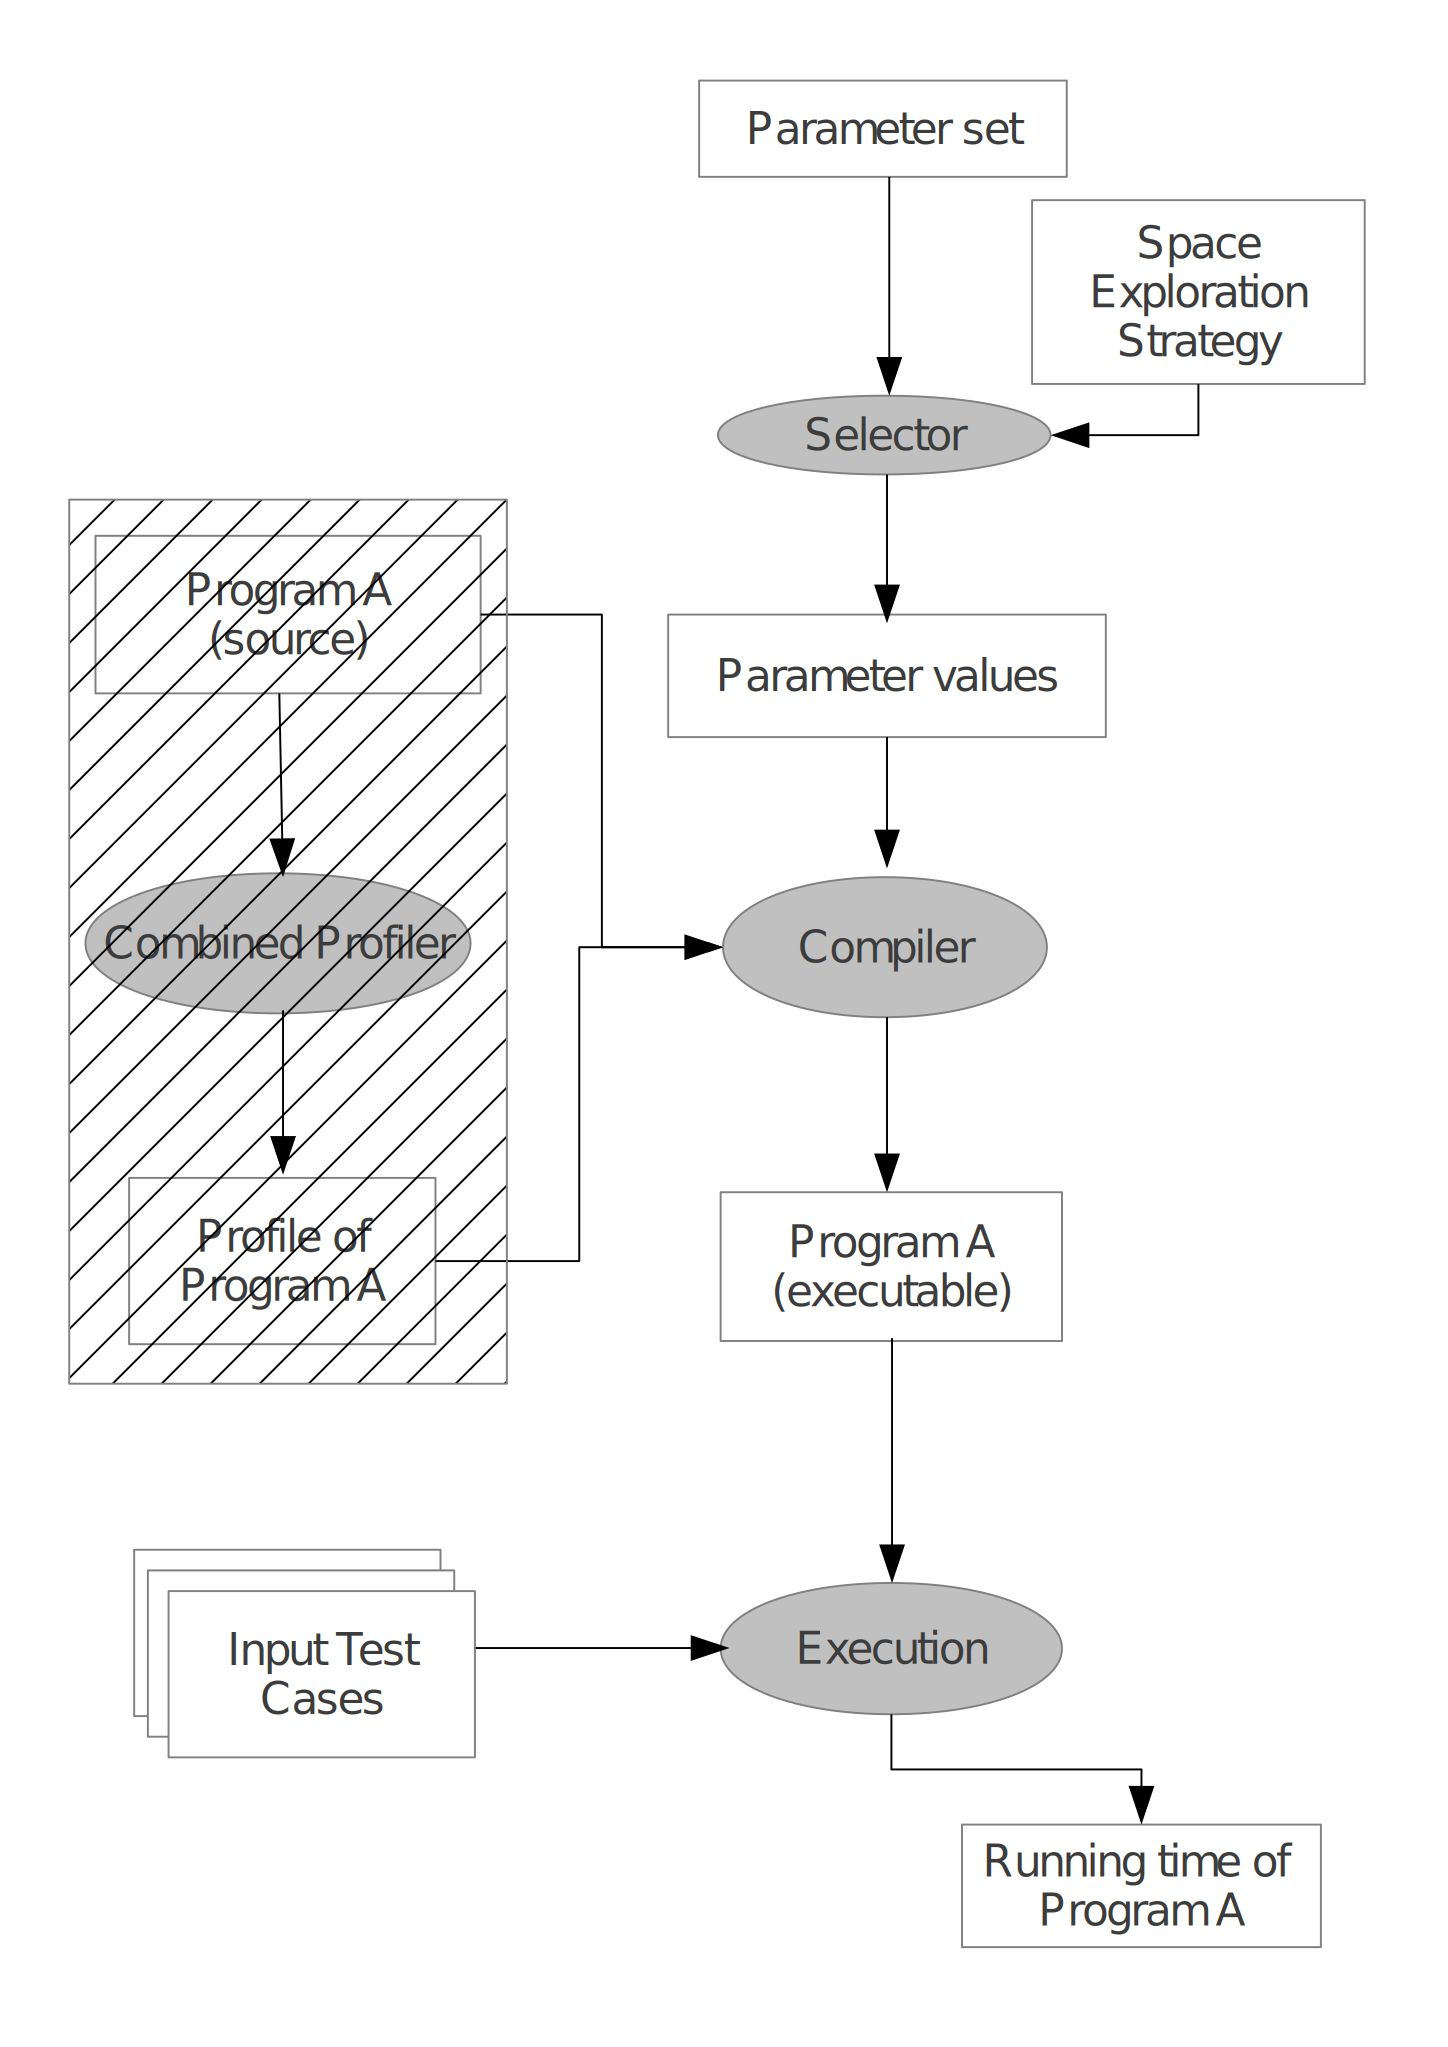
\includegraphics[height=12em]{Figures/CPview1}
      \end{minipage}
      \label{CP:simple}
    }
    \subfigure[Expanded view of the process] {
      \begin{minipage}[b]{0.45\textwidth}
        \centering
        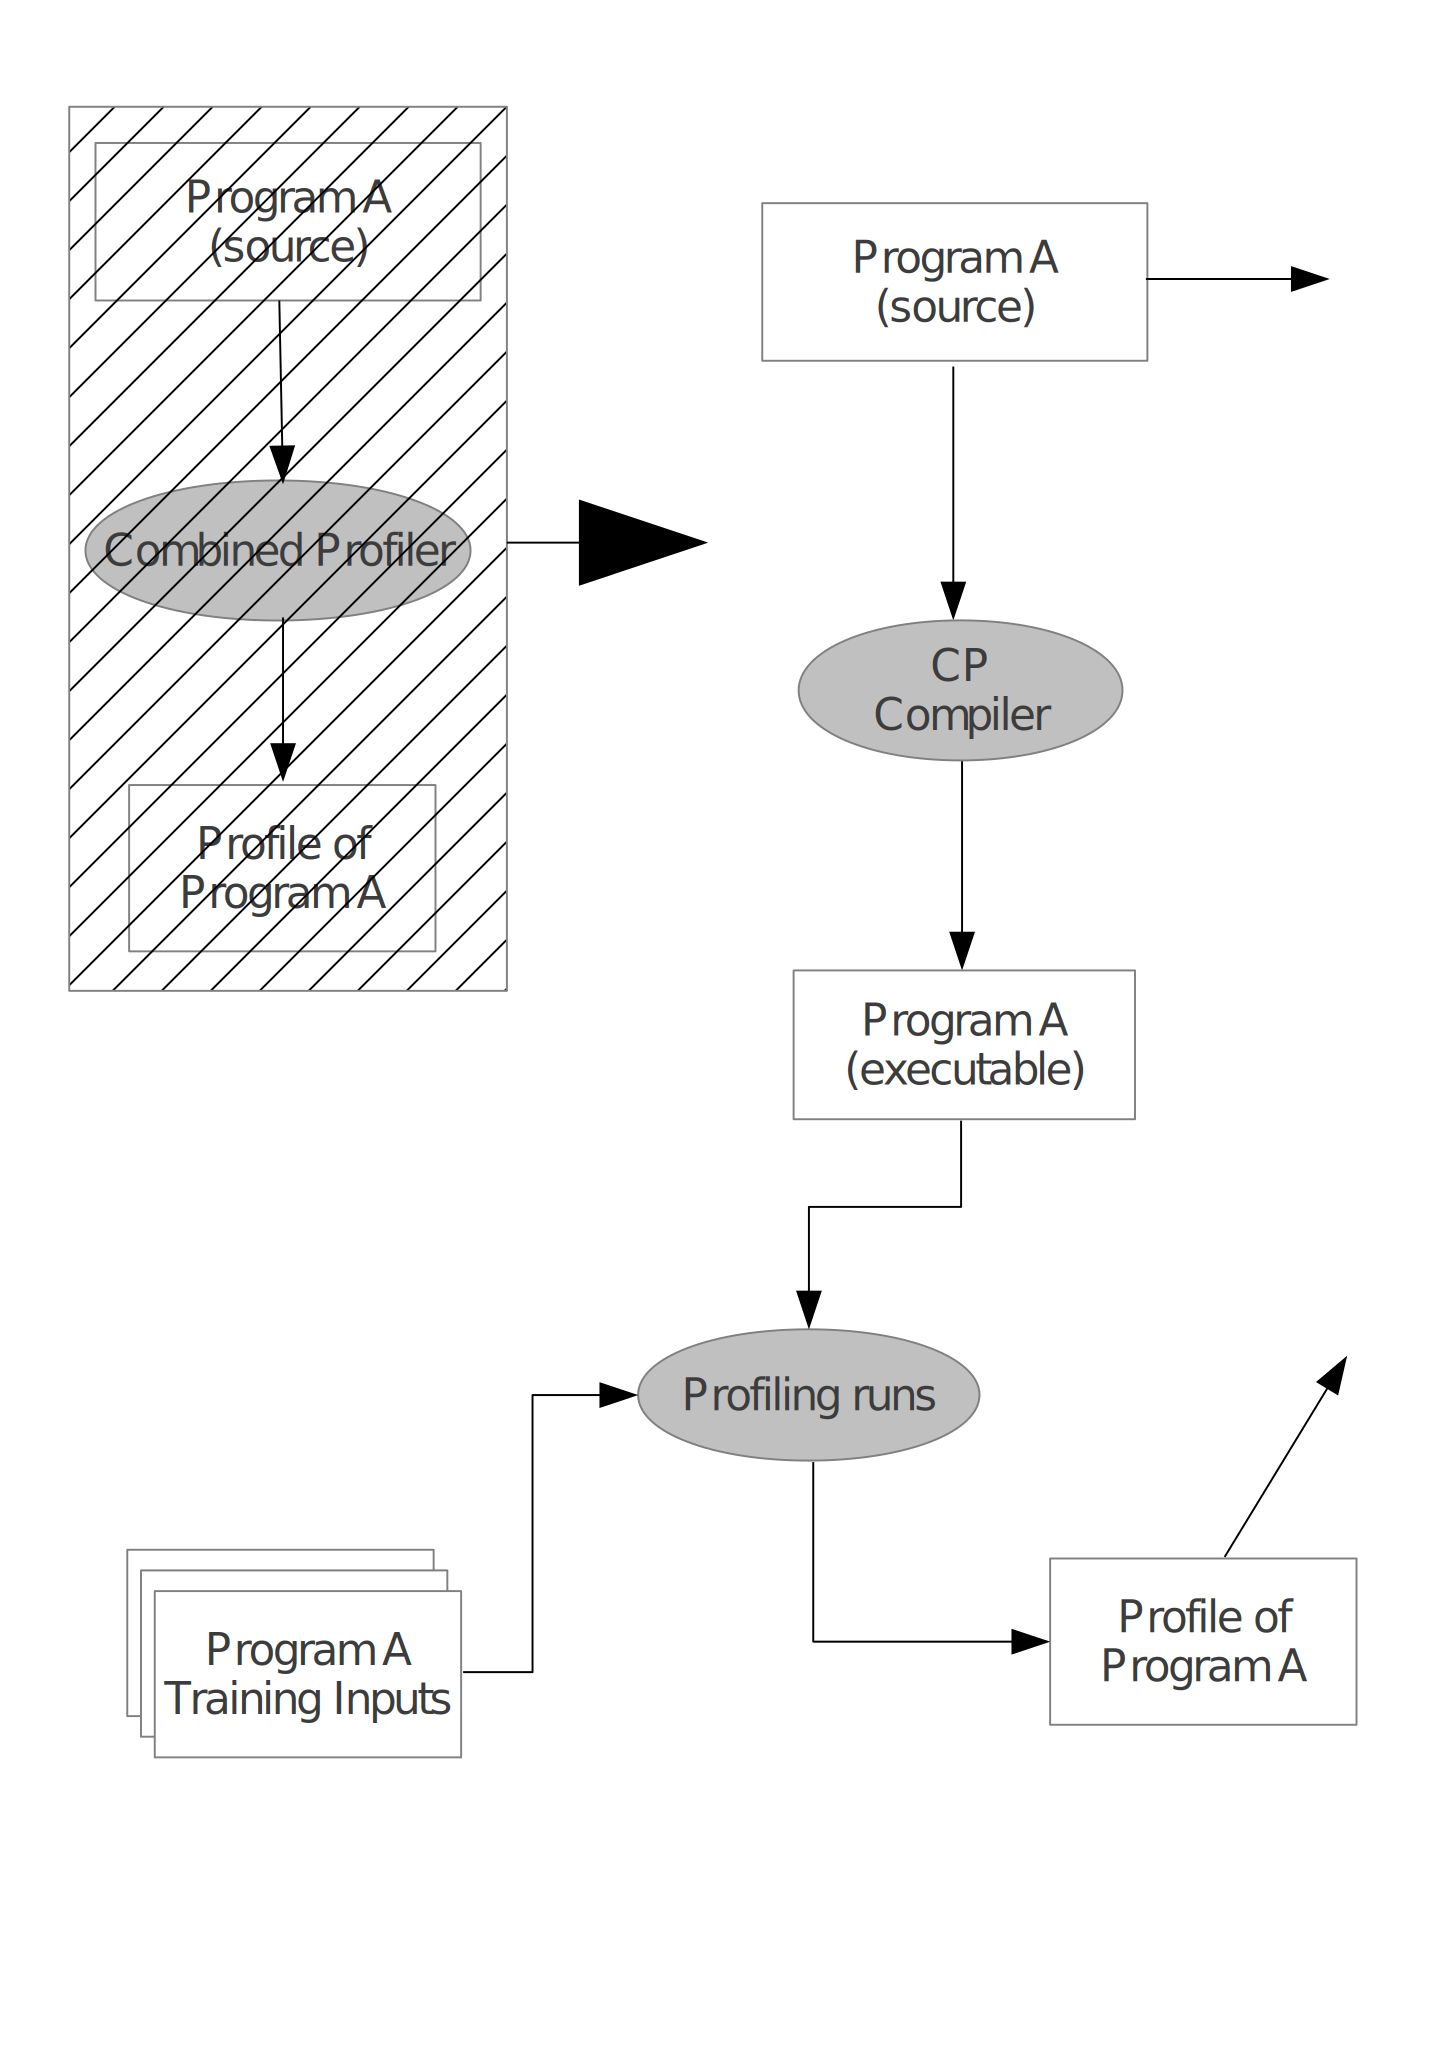
\includegraphics[height=12em]{Figures/CPview2}
      \end{minipage}
      \label{CP:expanded}
    }
  \end{minipage}
%    \vspace{1em}
%    \hrule
%    \vspace{1em}
  \caption{\CP\ compiler and the profile generation}
  \label{fig:CPview}
\end{figure}


In the case of parameter tuning, a point of measure is represented by
the set of parameter values of the compiler for the program under tuning
and its normalized value of the execution time for some test inputs. For
the machine learning case, a point of measure for throughput is the sum
of the execution times of each of the programs under test with its
associated parameter values. On the other hand for latency, a point of
measure is the geometric mean of the normalized values.

\subsection{Parameter Tuning}

Tuning compiler optimization options for a specific program is not an easy
task \cite{Zhong2009}. There exist some tools based on Genetic Algorithms,
Simulated Anealling \cite{Zhong2009}, Support Vector Machines \cite{SanchezCGO11},
etc. For the case of inlining a recently published research pointed to the
use of Neural Networks to induce effective inlining heuristics \cite{KulkarniCGO13}.
Parameter tuning is a proficuous area of research.

As illustrated if \refFigure{fig:genView}, our method can be used effetively
to tune compiler optimization options; in this research we made an empirical
evaluation of it in the inlining case.